%%%%%%%%%%%%%%%%%%%%%%%%%%%%%%%%%%%%%%%%%
% Wenneker Assignment
% LaTeX Template
% Version 2.0 (12/1/2019)
%
% This template originates from:
% http://www.LaTeXTemplates.com
%
% Authors:
% Vel (vel@LaTeXTemplates.com)
% Frits Wenneker
%
% License:
% CC BY-NC-SA 3.0 (http://creativecommons.org/licenses/by-nc-sa/3.0/)
% 
%%%%%%%%%%%%%%%%%%%%%%%%%%%%%%%%%%%%%%%%%

%----------------------------------------------------------------------------------------
%	PACKAGES AND OTHER DOCUMENT CONFIGURATIONS
%----------------------------------------------------------------------------------------

\documentclass[11pt]{scrartcl} % Font size

%%%%%%%%%%%%%%%%%%%%%%%%%%%%%%%%%%%%%%%%%
% Wenneker Assignment
% Structure Specification File
% Version 2.0 (12/1/2019)
%
% This template originates from:
% http://www.LaTeXTemplates.com
%
% Authors:
% Vel (vel@LaTeXTemplates.com)
% Frits Wenneker
%
% License:
% CC BY-NC-SA 3.0 (http://creativecommons.org/licenses/by-nc-sa/3.0/)
% 
%%%%%%%%%%%%%%%%%%%%%%%%%%%%%%%%%%%%%%%%%

%----------------------------------------------------------------------------------------
%	PACKAGES AND OTHER DOCUMENT CONFIGURATIONS
%----------------------------------------------------------------------------------------

\usepackage{amsmath, amsfonts, amsthm} % Math packages

\usepackage{listings} % Code listings, with syntax highlighting

\usepackage{xcolor} % Color extensions

\usepackage{cleveref} % Smarter referencing to labels {figures, tables, etc...}
\crefname{lstlisting}{listing}{listings}
\Crefname{lstlisting}{Listing}{Listings}

\usepackage[english]{babel} % English language hyphenation

\usepackage{graphicx} % Required for inserting images
\graphicspath{{graphics/}{./}} % Specifies where to look for included images (trailing slash required)

\usepackage{booktabs} % Required for better horizontal rules in tables

\usepackage{parskip} % Automatically insert newline

\usepackage{multirow} % allows multiple row in tabular environment

\numberwithin{equation}{section} % Number equations within sections (i.e. 1.1, 1.2, 2.1, 2.2 instead of 1, 2, 3, 4)
\numberwithin{figure}{section} % Number figures within sections (i.e. 1.1, 1.2, 2.1, 2.2 instead of 1, 2, 3, 4)
\numberwithin{table}{section} % Number tables within sections (i.e. 1.1, 1.2, 2.1, 2.2 instead of 1, 2, 3, 4)

\setlength\parindent{0pt} % Removes all indentation from paragraphs

\usepackage{enumitem} % Required for list customisation
\setlist{noitemsep} % No spacing between list items

%----------------------------------------------------------------------------------------
%	DOCUMENT MARGINS
%----------------------------------------------------------------------------------------

\usepackage{geometry} % Required for adjusting page dimensions and margins

\geometry{
	paper=a4paper, % Paper size, change to letterpaper for US letter size
	top=2.5cm, % Top margin
	bottom=3cm, % Bottom margin
	left=3cm, % Left margin
	right=3cm, % Right margin
	headheight=0.75cm, % Header height
	footskip=1.5cm, % Space from the bottom margin to the baseline of the footer
	headsep=0.75cm, % Space from the top margin to the baseline of the header
	%showframe, % Uncomment to show how the type block is set on the page
}

%----------------------------------------------------------------------------------------
%   Listing Style	
%----------------------------------------------------------------------------------------

\definecolor{ao}{rgb}{0.0, 0.5, 0.0}

\lstdefinestyle{CStyle}{
  language=C,                     % choose the language of the code
  numbers=left,                   % where to put the line-numbers
  stepnumber=1,                   % the step between two line-numbers.        
  numbersep=5pt,                  % how far the line-numbers are from the code
  backgroundcolor=\color{white},  % choose the background color. You must add \usepackage{color}
  commentstyle=\color{ao},
  keywordstyle=\color{blue},
  showspaces=false,               % show spaces adding particular underscores
  showstringspaces=false,         % underline spaces within strings
  showtabs=false,                 % show tabs within strings adding particular underscores
  tabsize=2,                      % sets default tabsize to 2 spaces
  captionpos=b,                   % sets the caption-position to bottom
  breaklines=true,                % sets automatic line breaking
  breakatwhitespace=true,         % sets if automatic breaks should only happen at whitespace
  title=\lstname,                 % show the filename of files included with \lstinputlisting;
}

%----------------------------------------------------------------------------------------
%	FONTS
%----------------------------------------------------------------------------------------

\usepackage[utf8]{inputenc} % Required for inputting international characters
\usepackage[T1]{fontenc} % Use 8-bit encoding

\usepackage{fourier} % Use the Adobe Utopia font for the document

%----------------------------------------------------------------------------------------
%	SECTION TITLES
%----------------------------------------------------------------------------------------

\usepackage{sectsty} % Allows customising section commands

\renewcommand\thesubsection{\alph{subsection}} % Alpha subsection numbering 
\renewcommand\thesubsubsection{\roman{subsubsection}} % roman subsubsection numbering

\sectionfont{\vspace{6pt}\centering\normalfont\scshape} % \section{} styling
\subsectionfont{\normalfont\bfseries} % \subsection{} styling
\subsubsectionfont{\normalfont\itshape} % \subsubsection{} styling
\paragraphfont{\normalfont\scshape} % \paragraph{} styling

%----------------------------------------------------------------------------------------
%	HEADERS AND FOOTERS
%----------------------------------------------------------------------------------------

\usepackage{scrlayer-scrpage} % Required for customising headers and footers

\ohead*{} % Right header
\ihead*{} % Left header
\chead*{} % Centre header

\ofoot*{} % Right footer
\ifoot*{} % Left footer
\cfoot*{\pagemark} % Centre footer
 % Include the file specifying the document structure and custom commands

%----------------------------------------------------------------------------------------
%	TITLE SECTION
%----------------------------------------------------------------------------------------

\title{	
	\normalfont\normalsize
	\textsc{Curtin University, Concurrent Systems}\\ % Your university, school and/or department name(s)
	\vspace{25pt} % Whitespace
	\rule{\linewidth}{0.5pt}\\ % Thin top horizontal rule
	\vspace{20pt} % Whitespace
	{\huge Lab report 3}\\ % The assignment title
	\vspace{12pt} % Whitespace
	\rule{\linewidth}{2pt}\\ % Thick bottom horizontal rule
	\vspace{12pt} % Whitespace
}

\author{\LARGE Nhan Dao} % Your name

\date{\normalsize\today} % Today's date (\today) or a custom date

\begin{document}

\pagenumbering{gobble}
\maketitle % Print the title
\newpage
\tableofcontents
\newpage

\pagenumbering{arabic}
%----------------------------------------------------------------------------------------
%	Monte Carlo method for estimating Pi using OpenMP
%----------------------------------------------------------------------------------------

\section{Monte Carlo method for approximating the value of $\pi$ in OpenMP}

\subsection{Compile and run the template code with a single thread, and thus verify that the serial
version is correct.}

\begin{figure}[ht]
    \centering
    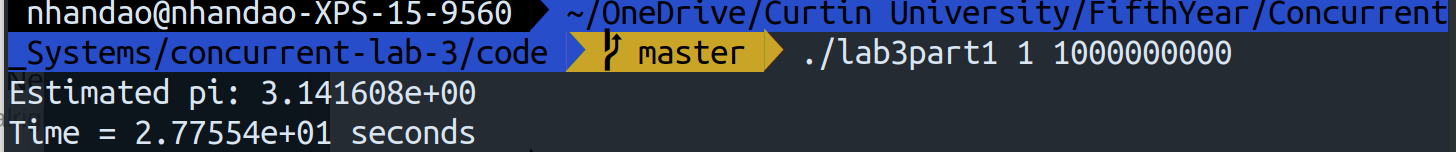
\includegraphics[width=\textwidth]{graphics/P1_a_terminal_output.png}
    \caption{Terminal output of execution of template code with a single thread}
    \label{fig:P1_a_term_out}
\end{figure}

\subsection{Parallelize the code for multi-threaded execution by ONLY adding OpenMP directives}

\vspace{0.5cm}
\lstinputlisting[
	style=CStyle,
	firstline=34, % First line of code
	lastline=48, % Lastl ine of code
	caption=Parallizing the code for multi-threaded execution (line 34-48 in lab3part1.c), % Caption above the listing
	label=lst:lab3part1a, % Label for referencing this listing
	frame=single, % Frame around the code listing
	showstringspaces=false, % Don't put marks in string spaces
	numbers=left, % Line numbers on left
	numberstyle=\normalsize % Line numbers styling
    ]{../code/lab3part1.c}
    
\subsubsection{At what point in the code new threads are forked and joined?}
The code is serial up until \emph{pragma}. At pragma, multiple threads are forked,
line 1 in \cref{lst:lab3part1a}. After the structured block (line 2 - 15), the slaves are joined with 
the master thread and execution resumes on the master thread.

\subsubsection{Which part of the code is executed by which threads?}
The total number of threads are comprised of one main thread, and the remainder are slave threads.
The main thread will run all code outside of the parallel enivornment. Master and slaves thread will 
run the section of code assigned by the OpenMP directives - line 2 - 15.

\subsubsection{Where barrires if any in terms of thread synchronization would be encountered,
and hence how the code achives parallelization}

Thread synchronization is needed to so reduction can be apply to the variable
\emph{number\_in\_circle} to avoid race condition. OpenMP's reduction basically
behaves similarly to a critical section in terms of synchronisation.


\subsection{Tabulate the speedup and efficiency for 1,2,4,8 threads.}

\begin{center}
\begin{tabular}{|| c | c | c | c ||}
	\hline
	Threads & Time (s) & Speedup & Efficiency (\%) \\ [0.5ex]
	\hline 
	1 & 20.356 & N/A & 100 \\
	2 & 10.376 & 1.962 & 98.10 \\
	4 & 5.908 & 3.476 & 86.90 \\
	8 & 3.498 & 5.819 & 72.74 \\
	\hline
\end{tabular}
\end{center}

\begin{figure}[ht]
	\centering
	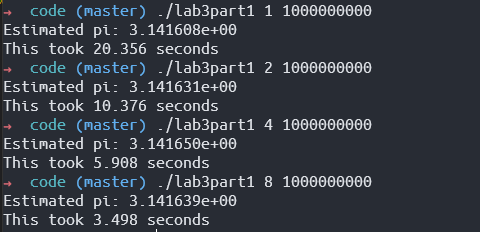
\includegraphics[width=\textwidth]{graphics/P1_c_terminal_output.PNG}
	\caption{Terminal output for execution with 1, 2, 4, 8 threads respectively for
	estimating $pi$ using Monte Carlo's method with $10^9$ samples}
	\label{fig:lab3part1c}
\end{figure}

\subsubsection{Do the result match your expectation? Why?}

The result matches our expectation. The speedup will increase as the number
of threads increase but will saturate at somepoint due to Amdahl's Law which
states that the parallel program is bounded by the section of code that 
can only be executed in serial. Hence, even though we are allocating more
threads, the efficiency decreases and we get a diminishing return due to this
fact. % Monte Carlo's extimation of Pi using OpenMP
\pagebreak
%----------------------------------------------------------------------------------------
% Trapezoidal rule to approximate area under a function
%----------------------------------------------------------------------------------------

\section{Trapezoidal rule to approximate area under $f(x)=x^4$ in OpenMP}

\subsection{Compile and run the template code with a single thread, for $a=0$,
$b=1$, $n=2^{30}$, and thus verify that the serial version is correct, also
checking the calculation by hand.}

\begin{figure}[ht]
	\centering
	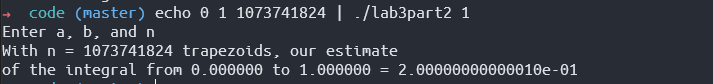
\includegraphics[width=\textwidth]{graphics/P2_a_terminal_output.PNG}
	\caption{Terminal output for $a=0$, $b=1$, $n=2^{30}$}
	\label{fig:P2_a}
\end{figure}


The following shows the calculation to compute by hand:
\vspace{1cm}
\begin{align*}
	\text{Area} &= \int_{0}^{1} x^4 \\
				&= \left[ \frac{x^5}{5} \right]^{1}_{0} \\
				&= \frac{1^5}{5} - \frac{0^5}{5} \\
				&= 0.2
\end{align*}

The computed integral using the trapezoidal rule equals to the answer worked out
by hand analytically using calculus (There is a negligible difference due to base
two floating-point numbers limitation to represent 1/20)

\subsection{Parallelize the code for multi-threaded execution by adding to 
it as few OpenMP directives as possible.}

\vspace{0.5cm}
\lstinputlisting[
	style=CStyle,
	firstline=63, % First line of code
	lastline=85, % Lastl ine of code
	caption=Parallizing the code for multi-threaded execution (line 56-78 in lab3part2.c), % Caption above the listing
	label=lst:lab3part2a, % Label for referencing this listing
	frame=single, % Frame around the code listing
	showstringspaces=false, % Don't put marks in string spaces
	numbers=left, % Line numbers on left
	numberstyle=\normalsize % Line numbers styling
	]{../code/lab3part2.c}
	
\subsubsection{At what points in the code new threads are forked and joined?}
Parallization occurs within the for loop though the use of OpenMP \emph{parallel 
for}. The \emph{for} pragma do not create a team of threads; instead they take
the team of threads that is active, and divide the loop iterations over them.

Since no threads were created prior to the pragma at line 17 in \cref{lst:lab3part2a},
this will be the point which new threads are forked. Threads are then joined
once the team of threads complete the iterations.

\subsubsection{Which parts of code is executed by which threads?}

The main thread will execute all the code outside the parallel region, I.E.
outside the for loop at line 17 in \cref{lst:lab3part2a}. Within the for loop,
OpenMP will take the team of thread that is active, and divide the loop iterations
over them which include the main thread, and any slaves thread.

\subsubsection{Where barriers if any in terms of thread synchronization would be
encountered, and hence how the code achieves parallelization?}

OpenMP creates a critical section and the values stored in  the private variable/s
(in this case it is the \emph{approx} variable) are reduced in the critical section.
This is synchronization that needs to happen to avoid race conditions between threads.

\subsection{Add timing statement to verify that the parallel solution runs faster
than the serial version. Tabulates the speedup and efficiency for 1, 2, 4, 8, threads.}

\begin{center}
\begin{tabular}{|| c | c | c | c ||}
	\hline
	Threads & Time (s) & Speedup & Efficiency (\%) \\ [0.5ex]
	\hline 
	1 & 3.439 & N/A & 100 \\
	2 & 1.920 & 1.791 & 89.557 \\
	4 & 1.252 & 2.747 & 68.67 \\
	8 & 0.754 & 4.561 & 57.013 \\
	\hline
\end{tabular}
\end{center}

\subsubsection{Do the result match the expectation? Why?}

As expected, the more threads will decrease the execution time, however, there
is a diminishing return such that the gain in speed from an increase in thread
diminishes as the thread number increase.

This is due to Amdahl's Law, which effectively state that their is an upper bound
in the speedup regardless the number of threads available unless virtually all of 
a serial program is parallelized. Since only the \emph{for} loop to compute 
the trapezoidal area is parallelized - 
the speed of the program is going to be very much bounded by the serial execution
of the non-parallel portion. 


\subsubsection{Explain why the output differs slightly from run to run for mulitple
thread?}

\begin{figure}[ht]
	\centering
	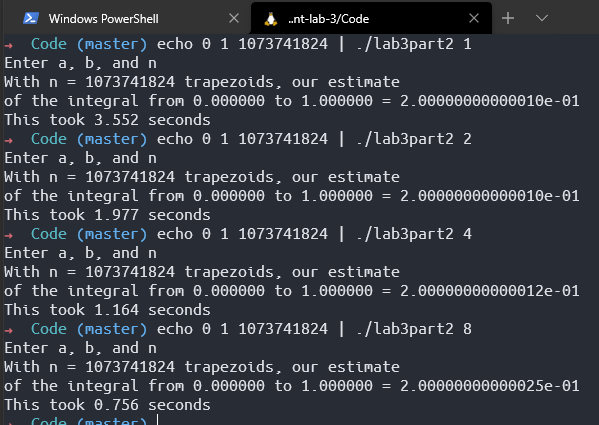
\includegraphics[width=\textwidth]{graphics/P2_c_terminal_output.PNG}
	\caption{Terminal output of execution for varying number of threads}
	\label{fig:lab3part2b}
\end{figure}

As seen in \cref{fig:lab3part2b}, the output differ slightly from run to run. 
The hypothesis is that the reduction is more accurate for higher thread count
due to the fact there is less floating-point precision loss because each thread
is approximating a smaller share of the area. In other words, for an integrand
of $\left[1, 0\right]$, a thread count of two will mean that each thread gets
50\% of the bound, whereas a thread count of 4 means each thread gets 25\% share
of the bound. A smaller bound would mean that there is less floating-point
precision loss as the reduction function is applied.


 % Trapezoidal rule to approximate area under a function f(x)=x^3 using OpenMP
\pagebreak
%----------------------------------------------------------------------------------------
% Parallel histogram generation using OpenMP
%----------------------------------------------------------------------------------------

\section{Parallel histogram generation using OpenMP}

\subsection{Compile and run the template code with a single thread to verify
that the serial version is correct}

\Cref{fig:lab3part3a} shows the terminal output for the execution of the template
code with one thread. 

\begin{figure}[ht]
	\centering
	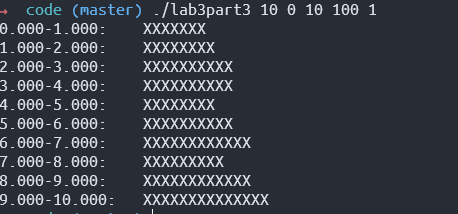
\includegraphics[width=\textwidth]{graphics/P3_a_terminal_output.PNG}
	\caption{Terminal output for execution with a single thread, using a 
	data range bewteeen 0 and 10, a total of 100 data points, and 10 equally
	spaced bins}
	\label{fig:lab3part3a}
\end{figure}

\subsection{Parallelize the code for multi-thread execution by ONLY adding OpenMP
directives}

\Cref{lst:lab3part3a} shows the changes within the template code to parallelize
by only adding OpenMP directives.

\vspace{0.5cm}
\lstinputlisting[
	style=CStyle,
	firstline=95, % First line of code
	lastline=119, % Lastl ine of code
	caption=Parallizing the code for multi-threaded execution (line 92-116 in lab3part3.c), % Caption above the listing
	label=lst:lab3part3a, % Label for referencing this listing
	frame=single, % Frame around the code listing
	showstringspaces=false, % Don't put marks in string spaces
	numbers=left, % Line numbers on left
	numberstyle=\normalsize % Line numbers styling
	]{../code/lab3part3.c}

\subsubsection{Explain how your code achieves parallelization.}

The first OpenMP directive is initializing the parallel environment
within the code block from line 3 to 25 in \cref{lst:lab3part3a}. This
directive will create a team of threads equal to the thread count specified
by the user, and all variables within that environment are within their own
scope in each thread (I.E stored within the stack of each thread).

The next directive divides the work of determining which data point falls
under which bin amongst the threads. It outputs the frequency of data point 
to a local histrogram counter in a form of an array. Here, the variable \emph{bin} must be 
declared private which makes a separte copy into each thread's stack. This is
done because we want to avoid race conditions for when multiple thread tries
to write to \emph{bin} at the same time.

The third and final \emph{for} directive sum up the local histogram counter
to the final output histogram. Here a nested for loop is used, because it needs
to iterate over each local histogram, and then each bin within the local histogram
to sum up the total histogram count.

\subsubsection{Describe at what points new threads are forked and joined and
which part of the code are executed by which threads.}

New threads are forked when the parallel environment begins (line 2 in 
\cref{lst:lab3part3a}) and they are joined once the parallel environment ends
(line 25 \cref{lst:lab3part3a}). Within the parallel environment, work
are divided amongst the threads, I.E, through the use of the \emph{for} pragma.
Any code outside of the parallel environment are run in serial by the main thread.

\subsection{Tabulate the speedup and efficiency for 1,2,4,8 threads using a data
range between 0 and 10, a total of $10^7$ data points, and 10 equally spaced bins}

\begin{center}
\begin{tabular}{|| c | c | c | c ||}
	\hline
	Threads & Time (s) & Speedup & Efficiency (\%) \\ [0.5ex]
	\hline 
	1 & 0.474 & N/A & 100 \\
	2 & 0.295 & 1.607 & 80.34 \\
	4 & 0.227 & 2.088 & 52.20 \\
	8 & 0.195 & 2.431 & 30.38\\
	\hline
\end{tabular}
\end{center}

\begin{figure}[ht]
	\centering
	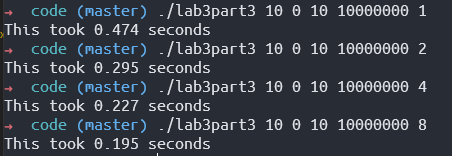
\includegraphics[width=\textwidth]{graphics/P3_c_terminal_output.PNG}
	\caption{Terminal output for execution with 1, 2, 4, 8 threads respectively,
	using a data range bewteeen 0 and 10, a total of $10^7$ data points, and 10 equally
	spaced bins.}
	\label{fig:lab3part3c}
\end{figure} % Parallel histogram generation using OpenMP
\pagebreak
%----------------------------------------------------------------------------------------
% Parallel count sort
%----------------------------------------------------------------------------------------

\section{Parallel Count Sort using OpenMP}
 % Parallel count sort using OpenMP

\end{document}
